\chapter{SP2-CU2 Consultar paquetes de Unidad de Aprendizaje del Jefe de Innovación}

\begin{UseCase}{SP2-CU2}{ Consultar paquetes de Unidad de Aprendizaje del Jefe de Innovación}{El usuario jefe de desarrollo e innovación curricular podrá consultar los paquetes que contienen las unidades de aprendizaje de la unidad académica correspondiente.}
		\UCitem{Versión}{\color{Gray}1.0}
		\UCitem{Autor}{\color{Gray}Parra Garcilazo Cinthya Dolores}
		\UCitem{Supervisa}{\color{Gray}}
		\UCitem{Actor}{\hyperlink{Usuario}{Jefe de Desarrollo e Innovación Curricular}}
		\UCitem{Propósito}{Conocer el estado de los paquetes de las unidades académicas que fueron enviadas a la DES para su revisión.}
		\UCitem{Entradas}{Las entradas para consultar un paquete de unidades de aprendizaje son:
          \begin{itemize}
          	\item Unidad Académica
            \item Programa académico
		\item Semestre
		\item Número de revisión
          \end{itemize}
        }
		\UCitem{Origen}{Teclado, mouse.}
		\UCitem{Salidas}{
        	\begin{itemize}
        	   \item MSG25. Ha ocurrido un error con la base de datos.

        	\end{itemize}
        }
		\UCitem{Destino}{Pantalla.}
		\UCitem{Precondiciones}{ 
			\begin{itemize}
        	   \item El mapa curricular de la unidad académica debe haber sido registrado previamente.
		   \item Los paquetes deben ser enviados por la unidad académica correspondiente.

        	\end{itemize}
		}
		\UCitem{Postcondiciones}{Se visualiza el paquete de unidades de aprendizaje de un semestre en particular, elegido por el usuario.}
		\UCitem{Errores}{No hay conexión con la base de datos.}
		\UCitem{Estado}{Aprobado.}
		\UCitem{Observaciones}{}
\end{UseCase}

%--------------------------- CU TRAYECTORIA PRINCIPAL -------------------------
\begin{UCtrayectoria}{Principal}


    \UCpaso Muestra la interfaz de usuario \IUref{SP2-IU-ConsultaPaquete}
    \UCpaso [\UCactor] Selecciona el select de unidad académica
    \UCpaso Consulta la base de datos\hyperref[SP2-CU5-A]{Trayectoria A}.
    \UCpaso Despliega las unidades académicas que se encuentran en revisión.
    \UCpaso [\UCactor] Selecciona una opción de unidades académicas.
    \UCpaso Consulta los programas académicos que se encuentren en estado de revisión de esa unidad académica en la base de datos. \hyperref[SP2-CU5-A]{Trayectoria A}.
    \UCpaso Despliega los resultados de la consulta de programas académicos.
    \UCpaso [\UCactor] Selecciona un programa académico.
    \UCpaso Consulta los semestres que se encuentren en estado de revisión de esa unidad académica en la base de datos. \hyperref[SP2-CU5-A]{Trayectoria A}.
    \UCpaso Despliega los resultados de los números de revisión.
    \UCpaso [\UCactor] Selecciona un número de revisión.
    \UCpaso [\UCactor] Presiona el botón. \IUbutton {Buscar}
    \UCpaso Consulta las unidades de aprendizaje que pertenezcan a esa unidad académica, programa académico, semestre y número de revisión.
    \UCpaso Muestra la interfaz de usuario \IUref{SP2-IU-GestionEncargado}.

\end{UCtrayectoria}


%------------------------ CU TRAYECTORIA ALTERNARIVA A -------------------------
\label{SP2-CU5-A}
\begin{UCtrayectoriaA}{A}{No hay conexión con la base de datos.}
    \UCpaso Muestra el mensaje MSG25. Ha ocurrido un error con la base de datos.
    \UCpaso[\UCactor] Presiona el botón \IUbutton {Aceptar}
\end{UCtrayectoriaA}

%------------------------ Pantallas de este caso de uso -------------------------
\chapter{Pantallas}
 \begin{figure}
  \centering
    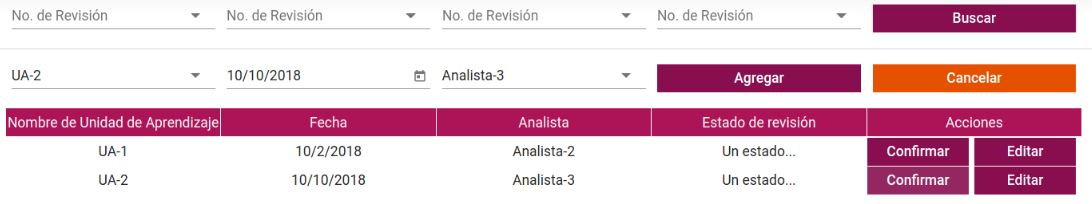
\includegraphics[width=0.7\textwidth]{DCU/SP2/Pantallas/ConsultaPaquete}
  \caption{SP2-IU-ConsultaPaquete}
  \label{SP2-IU-ConsultaPaquete}
\end{figure}

 \begin{figure}
  \centering
    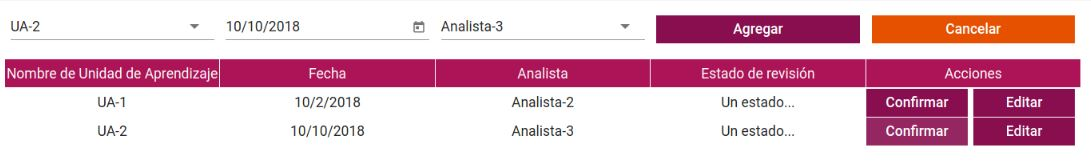
\includegraphics[width=0.7\textwidth]{DCU/SP2/Pantallas/GestionEncargado}
  \caption{SP2-IU-GestionEncargado}
  \label{SP2-IU-GestionEncargado}
\end{figure}


